\section{Results and Economic Interpretation}
\label{sec:results}
\subsection{Net performance relative to the investment benchmarks}
Table~\ref{tab:headline} reports final-period results at 5 basis points per one-way trade. Ridge timing earns \RidgeCAGR{} CAGR, compared with \BHCAGR{} for buy-and-hold and 3.69\% for MA20. Its arithmetic annual return is 7.56\%, annualized volatility is 15.72\%, and Sharpe is \RidgeSharpe{}. The passive strategy has a higher return and Sharpe, while MA20 has the lowest volatility and growth.

\begin{table}[!htbp]
\centering\small
\caption{Final evaluation, 2022--2025: performance after 5 bps single-side costs.}
\label{tab:headline}
\begin{tabular}{lrrr}
\toprule
Metric & Ridge & MA20 & Buy-and-hold \\
\midrule
CAGR (\%) & 6.54 & 3.69 & 11.18 \\
Arithmetic return (\%) & 7.56 & 4.22 & 12.27 \\
Volatility (\%) & 15.72 & 10.83 & 18.31 \\
Sharpe ($r_f=0$) & 0.481 & 0.389 & 0.670 \\
Max. drawdown (\%) & -22.20 & -19.14 & -26.28 \\
Total return (\%) & 28.63 & 15.52 & 52.38 \\
Equity exposure (\%) & 69.36 & 65.27 & 100.00 \\
One-way turnover & 246 & 102 & 2 \\
\bottomrule
\end{tabular}

\tabnote{All strategies use the same 1,002 opening-to-opening intervals, initial capital, dividend convention, and liquidation date. Returns and volatility are annualized except for total return. Equity exposure is the proportion of intervals invested.}
\end{table}

\begin{figure}[!htbp]
\centering
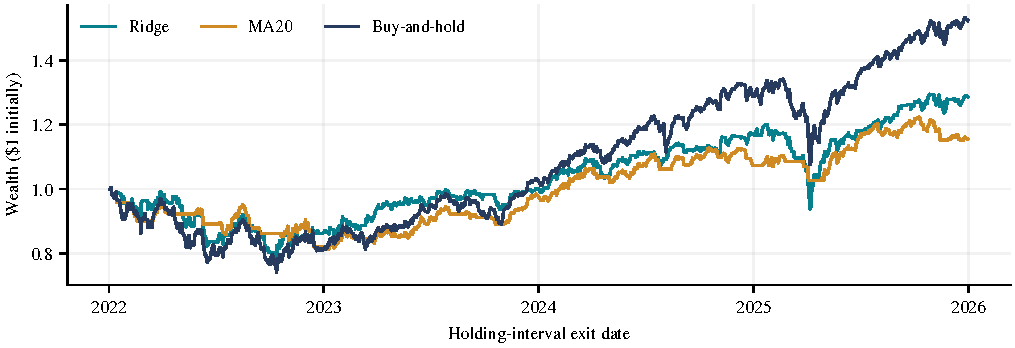
\includegraphics[width=.96\textwidth]{figures/wealth.pdf}
\caption{Cumulative net wealth from one unit of initial capital. Entry and final liquidation are included in every path. Source: \code{output/tables/test_path_*.csv}.}
\label{fig:wealth}
\end{figure}

The terminal wealth values are 1.286 for Ridge, 1.155 for MA20, and 1.524 for buy-and-hold. Figure~\ref{fig:wealth} shows how the difference develops over the full holding period. Ridge reduces losses during parts of 2022, but subsequently participates in fewer of the positive equity returns. Its lead over MA20 does not translate into an advantage over the passive alternative.

The magnitude of the trade-off is economically important. Ridge's CAGR is 4.64 percentage points below buy-and-hold, while its maximum drawdown is 4.08 percentage points smaller in absolute magnitude. These quantities describe different aspects of the wealth path, so the drawdown improvement does not offset the growth difference automatically. The remaining results examine the prediction, cost, and exposure components separately.

\subsection{Transaction costs and the implementation gap}
\label{sec:costresults}
At zero cost, Ridge earns 9.88\% CAGR and a Sharpe of 0.678. Buy-and-hold earns 11.20\% and 0.672. Thus gross risk-adjusted performance is numerically close, although gross growth is already lower for the timing rule. At 5 bps, Ridge's Sharpe falls to 0.481; at 10 bps it falls to 0.284. Figure~\ref{fig:cost} and Table~\ref{tab:costridge} isolate this change while keeping the position path fixed.

\begin{figure}[!htbp]
\centering
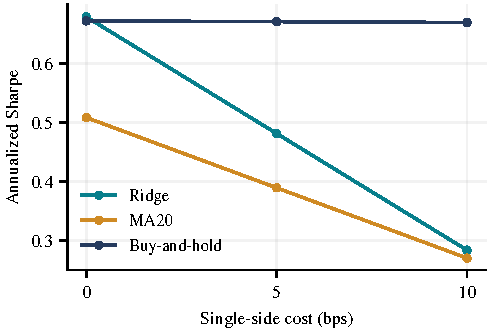
\includegraphics[width=.64\textwidth]{figures/cost_sharpe.pdf}
\caption{Sharpe sensitivity to the single-side fee. The same forecasts and positions are priced at 0, 5, and 10 bps.}
\label{fig:cost}
\end{figure}

\begin{table}[!htbp]
\centering\small
\caption{Ridge and buy-and-hold at the three declared cost levels.}
\label{tab:costridge}
\begin{tabular}{lrrrr}
\toprule
bps & Ridge CAGR (\%) & Sharpe & BH CAGR (\%) & BH Sharpe \\
\midrule
0 & 9.88 & 0.678 & 11.20 & 0.672 \\
5 & 6.54 & 0.481 & 11.18 & 0.670 \\
10 & 3.29 & 0.284 & 11.15 & 0.669 \\
\bottomrule
\end{tabular}

\tabnote{CAGR values are percentages; BH denotes buy-and-hold. The complete three-strategy comparison is in Appendix~\ref{app:fullresults}.}
\end{table}

Ridge incurs 246 charged one-way trade units, equivalent to 123 completed entry--exit round trips. Annualized turnover is 61.87 one-way units. MA20 incurs 102 units, and buy-and-hold incurs two. The contrast explains why the passive strategy's cost curve is almost flat while Ridge's declines sharply.

Equation~\eqref{eq:drag} gives the exact wealth reduction from the assumed fee. For Ridge,
\begin{equation}
\frac{V_N(0.0005)}{V_N(0)}=(0.9995)^{246}=0.884236.
\end{equation}
The fee removes 11.58\% of terminal gross wealth, corresponding to 3.094\% annualized log-wealth drag. MA20's corresponding drag is 1.283\%, and buy-and-hold's is 0.025\% (Table~\ref{tab:logdrag}). The arithmetic annual return for Ridge falls from 10.66\% gross to 7.56\% net. These calculations quantify an implementation mechanism that is distinct from a change in the forecasting model.

\begin{table}[!htbp]
\centering\small
\caption{Cost attribution at 5 bps using the exact turnover identity.}
\label{tab:logdrag}
\begin{tabular}{lrrr}
\toprule
Strategy & $K$ & Net/gross wealth & Annual log drag (\%) \\
\midrule
Ridge & 246 & 0.884236 & 3.094 \\
MA20 & 102 & 0.950267 & 1.283 \\
Buy-and-hold & 2 & 0.999000 & 0.025 \\
\bottomrule
\end{tabular}

\tabnote{Annual log drag is $-(252K/N)\log(1-c)$; it is not the percentage-point change in CAGR.}
\end{table}

The entry scores help explain why frequent switches are expensive. There are 123 cash-to-SPY entries, with a median predicted holding return of 4.17 bps; 56.10\% of entry scores are below 5 bps. Each invested run lasts 5.65 holding intervals on average. A forecast of one interval's return therefore triggers a position whose eventual duration is determined by subsequent signs. The initial score measures neither the complete run's expected return nor its total fee burden.

For scale, a position entered and liquidated after one interval needs an asset return of $(1-c)^{-2}-1$, or approximately 10.01 bps at $c=0.0005$, just to recover its two trading charges. A multi-interval run spreads those charges over a longer period. This accounting comparison explains why a positive score alone can be insufficient for profitable implementation: the zero threshold responds to the forecast's sign, whereas fees depend on position transitions and eventual exit. The recorded entry scores and holding durations locate that mismatch in the actual trading path.

\subsection{Forecast quality and the scale of the trading signal}
The model's squared-error performance does not improve on the rolling historical mean. Its MSE is 0.00013365, compared with 0.00013293 for the reference, giving $R^2_{\mathrm{OOS}}=\OOSRsquared{}$. The prediction error is approximately 0.54\% higher than the baseline error. The forecast--outcome correlation is 0.0295.

Equation~\eqref{eq:meanadjustment} allows the incremental forecast to be assessed directly. Let $m_i$ be the historical-mean forecast, $\delta_i=\widehat y_i-m_i$ the feature adjustment, and $e_i=y_i-m_i$ the baseline error. The exact sample identity is
\begin{equation}
\operatorname{MSE}(\widehat y)-\operatorname{MSE}(m)
=\overline{\delta^2}-2\overline{e\delta}.
\label{eq:mseparts}
\end{equation}
In squared-basis-point units, the first term is 162.24 and the second is 90.28, leaving an increase of 71.96. The adjustment aligns positively with the baseline error, but its squared magnitude exceeds the error reduction from that alignment. The negative out-of-sample $R^2$ therefore reflects an adjustment that is too variable relative to its realized predictive contribution, rather than an absence of any positive forecast association.

\begin{table}[!htbp]
\centering\small
\caption{Prediction diagnostics for the frozen final-period forecasts.}
\label{tab:prediction}
\begin{tabular}{@{}lr@{}}
\toprule
Measure & Value \\
\midrule
Model MSE & 0.00013365 \\
Historical-mean MSE & 0.00013293 \\
$R^2_{\mathrm{OOS}}$ & -0.00541 \\
Direction accuracy (\%) & 51.20 \\
Positive-return fraction (\%) & 53.49 \\
Forecast--outcome correlation & 0.0295 \\
Mean absolute forecast (bps) & 9.92 \\
Forecasts within 5 bps of zero (\%) & 37.33 \\
\bottomrule
\end{tabular}

\tabnote{The reference mean uses the same mature training window and monthly update schedule as Ridge. The positive-return fraction is the accuracy of an always-positive direction forecast.}
\end{table}

Directional accuracy is 51.20\%, below the 53.49\% fraction of positive underlying intervals. The model predicts a positive return in 695 of 1,002 cases. Of those invested cases, 371 realize positive returns; among 307 cash cases, 142 realize non-positive returns. The model therefore has no direction-accuracy advantage over an always-positive forecast in this sample. The portfolio comparison additionally weights each outcome by its magnitude and accounts for the trades.

\begin{figure}[!htbp]
\centering
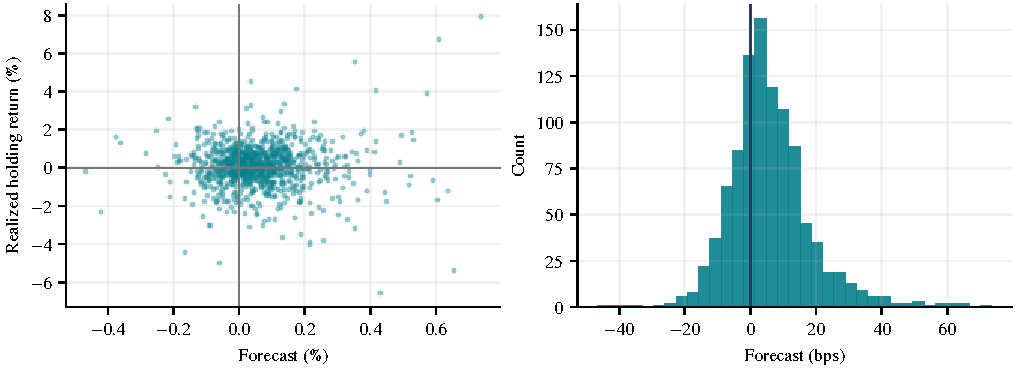
\includegraphics[width=.96\textwidth]{figures/predictions.pdf}
\caption{Forecast scale and realized returns. Left: each point is a predicted and realized holding return. Right: the distribution of forecast scores, with the trading threshold at zero.}
\label{fig:predictions}
\end{figure}

Figure~\ref{fig:predictions} shows the scale mismatch. The standard deviation of forecasts is 12.80 bps, versus 115.33 bps for realized holding returns. The mean absolute forecast is 9.92 bps, and 37.33\% of forecasts are within 5 bps of zero. Under the binary rule, those small positive forecasts receive the same allocation as the largest positive forecasts. When a prediction crosses zero, the entire portfolio changes between SPY and cash. The score distribution therefore helps connect modest predictive variation to large one-way trade amounts.

The returns held and missed provide another useful decomposition. Mean SPY return is 6.097 bps in invested intervals and 2.121 bps in cash intervals (Table~\ref{tab:conditional}). Although the invested subset has the higher mean, the excluded subset also has positive average returns. Writing $p$ for the invested fraction, the full asset mean is
\begin{equation}
\overline y=p\,\overline y_{\mathrm{invested}}+(1-p)\,\overline y_{\mathrm{cash}},
\end{equation}
whereas the strategy's gross mean is only $p\,\overline y_{\mathrm{invested}}$. With $p=0.6936$, the forgone cash-interval asset returns account for about 1.64 percentage points of arithmetic annual return before fees. Gross Ridge return is therefore 10.66\% rather than the passive 12.30\%, even though the invested subset has a higher mean return.

\begin{table}[!htbp]
\centering\small
\caption{Realized asset returns grouped by the model's position.}
\label{tab:conditional}
\begin{tabular}{lrrrr}
\toprule
Ridge decision & Count & Mean $y$ (bps) & SD (bps) & Positive (\%) \\
\midrule
Invested intervals & 695 & 6.097 & 118.821 & 53.38 \\
Cash intervals & 307 & 2.121 & 107.137 & 53.75 \\
\bottomrule
\end{tabular}

\tabnote{The cash row records the SPY returns forgone while the portfolio held zero-interest cash. Values describe underlying asset returns before portfolio fees.}
\end{table}

The same saved paths reconcile the net arithmetic return gap exactly. Write $F_i^s$ for strategy $s$'s gross return minus its net return, including any final liquidation charge. Since gross buy-and-hold earns $y_i$ and gross Ridge earns $w_i y_i$,
\begin{equation}
252\bigl(\overline R^{\mathrm{BH}}-\overline R^{\mathrm{Ridge}}\bigr)
=252\,\overline{(1-w)y}
+252\bigl(\overline F^{\mathrm{Ridge}}-\overline F^{\mathrm{BH}}\bigr).
\label{eq:netgap}
\end{equation}
Table~\ref{tab:gap} gives the corresponding quantities. Missing positive equity returns costs 1.64 percentage points annually; incremental fees cost another 3.07 points. Together they account for the 4.71-point arithmetic shortfall. Fees explain about 65.20\% of that gap, with reduced participation explaining the remainder. This is an additive return attribution; the 4.64-point CAGR gap additionally reflects compounding.

\begin{table}[!htbp]
\centering\small
\caption{Reconciliation of buy-and-hold's net arithmetic return advantage.}
\label{tab:gap}
\begin{tabular}{@{}lr@{}}
\toprule
Component & Annual gap (pp) \\
\midrule
Equity returns forgone during cash intervals & 1.64 \\
Incremental fee drag relative to buy-and-hold & 3.07 \\
Total net arithmetic return gap & 4.71 \\
\bottomrule
\end{tabular}

\tabnote{Values are annual percentage points, calculated from the same 1,002 saved holding intervals at 5 bps. Fee drag is measured in realized interval returns.}
\end{table}

\subsection{Risk, drawdown, and market participation}
Ridge's 15.72\% annualized volatility is below buy-and-hold's 18.31\%, and maximum drawdown is \RidgeMDD{} rather than \BHMDD{}. MA20 has lower volatility and drawdown still, at 10.83\% and $-19.14\%$, but earns the lowest CAGR. Figure~\ref{fig:drawdown} makes the growth--risk trade-off visible over time.

\begin{figure}[!htbp]
\centering
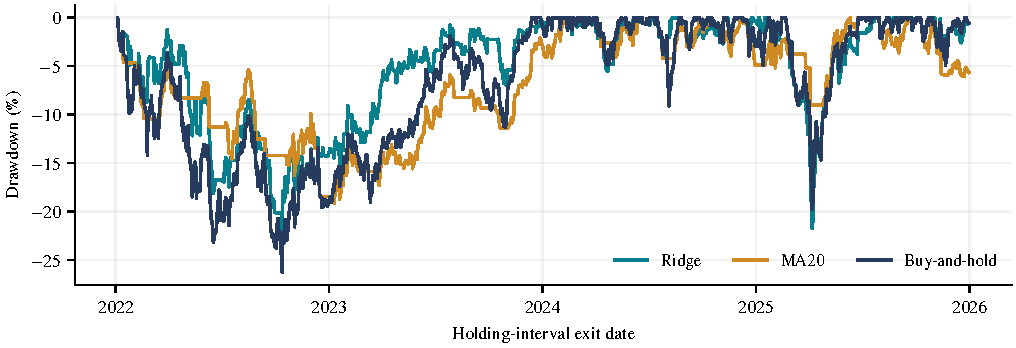
\includegraphics[width=.96\textwidth]{figures/drawdown.pdf}
\caption{Net drawdowns from the running wealth peak, including the initial investment.}
\label{fig:drawdown}
\end{figure}

Average market participation is 69.36\% for Ridge and 65.27\% for MA20. Figure~\ref{fig:exposure} shows the variation in monthly participation. These are averages of binary daily positions: a month with 70\% exposure means the strategy was fully invested during roughly 70\% of its holding intervals, not that it maintained a daily fractional position.

\begin{figure}[!htbp]
\centering
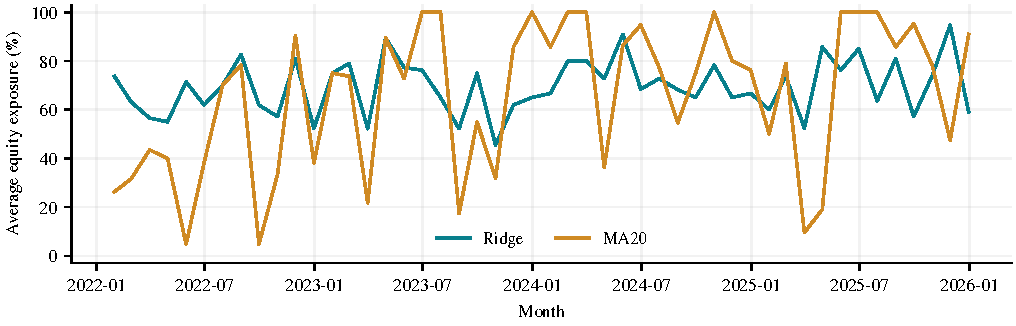
\includegraphics[width=.96\textwidth]{figures/exposure.pdf}
\caption{Monthly mean equity exposure for the two timing rules. Buy-and-hold remains fully invested throughout.}
\label{fig:exposure}
\end{figure}

The saved ex post exposure diagnostic places a constant gross fraction of 69.36\% in SPY. It has 8.03\% CAGR, 12.70\% volatility, and 0.672 Sharpe. For a fixed positive fraction $p$ and zero cash return, multiplying every asset return by $p$ scales its arithmetic mean and standard deviation equally, leaving gross Sharpe unchanged. This explains how lower equity participation alone can lower volatility. Ridge's observed risk reduction should therefore be evaluated alongside the lower net Sharpe, rather than treated as a separate timing success. The diagnostic's construction is discussed in Section~\ref{sec:limitations}.

Binary timing does not reduce each day's market position proportionally. It retains the full return during invested intervals and replaces it with zero during cash intervals. The underlying return standard deviation is 118.82 bps in the invested subset and 107.14 bps in the cash subset. Thus the observed allocation does not concentrate its equity exposure in the lower-volatility subset. Consistently, gross Ridge volatility is 15.71\%, above the constant-fraction diagnostic's 12.70\% despite matching its average exposure. The lower full-sample risk relative to a fully invested portfolio is closely connected to time spent in cash; the conditional return figures supply no corresponding evidence of successful low-risk interval selection.

\subsection{Annual performance and rolling coefficients}
Figure~\ref{fig:annual} presents annual net returns and Sharpe ratios. Ridge loses 13.80\% in 2022, compared with 18.82\% for buy-and-hold. It then earns 16.15\%, 16.90\%, and 9.88\% in 2023--2025, below the corresponding passive returns of 27.09\%, 25.40\%, and 17.79\%. The reduction in the first year's loss does not compensate for the subsequent participation gap. The complete annual metrics are given in Appendix~\ref{app:fullresults}.

\begin{figure}[!htbp]
\centering
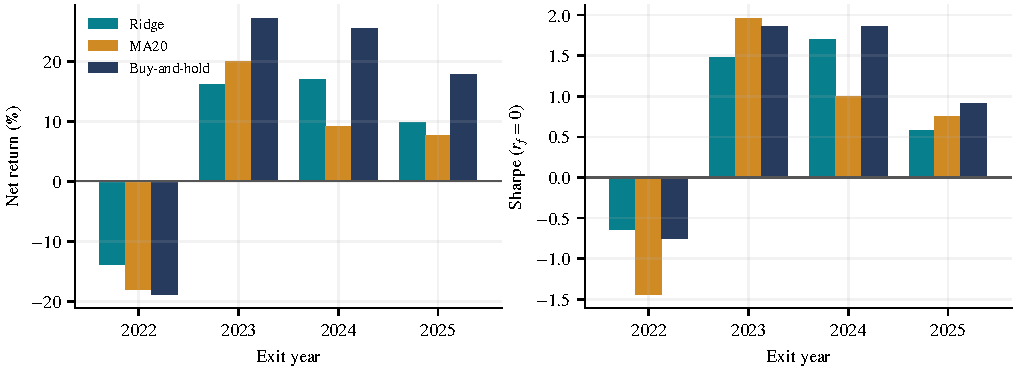
\includegraphics[width=.96\textwidth]{figures/annual.pdf}
\caption{Calendar-year net returns and Sharpe ratios at 5 bps. Annual returns compound the continuous portfolio path without year-end liquidation.}
\label{fig:annual}
\end{figure}

Annual risk also varies. Ridge volatility is about 20.11\% in 2022, 10.60\% in 2023, 9.47\% in 2024, and 19.59\% in 2025. The 2025 within-year maximum drawdown is 21.75\%, versus 19.76\% for buy-and-hold. Thus the smaller full-period drawdown does not describe a uniform year-by-year reduction in losses. Average exposure remains between 65.60\% and 73.02\%, so the strategy continues to hold substantial equity risk in each year.

\begin{figure}[!htbp]
\centering
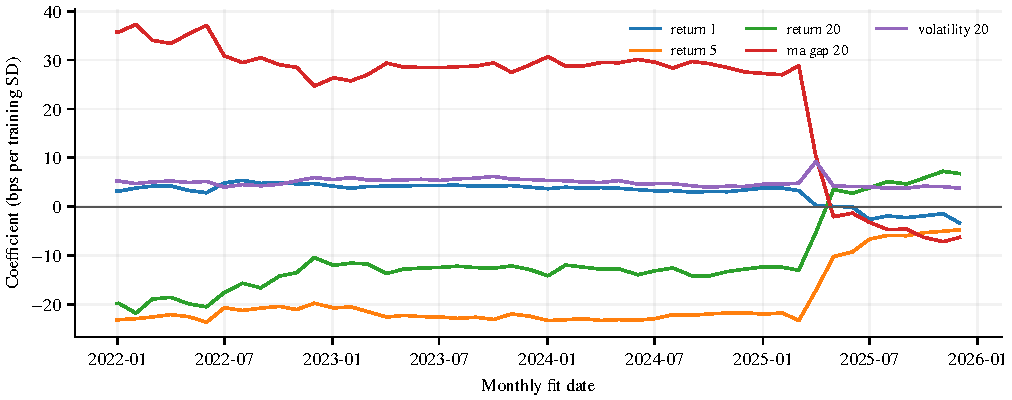
\includegraphics[width=.96\textwidth]{figures/coefficients.pdf}
\caption{Monthly Ridge coefficients on training-standardized features, in bps per training standard deviation. Each curve contains the 49 recorded final-period fits.}
\label{fig:coefficients}
\end{figure}

Figure~\ref{fig:coefficients} relates the daily decisions to the fitted predictive relationship. The five-session return coefficient is negative in all 49 fits, while the volatility coefficient is positive throughout. Their mean standardized coefficients are $-19.59$ and $4.96$ bps. The moving-average gap has a mean coefficient of 23.81 bps and changes sign once. Several coefficient paths change substantially around the second quarter of 2025, showing that the scheduled rolling procedure can alter its estimated relationship even with a fixed penalty and feature set.

Because the model combines several overlapping trend measures, the investment decision depends on their sum and the intercept. For example, the positive moving-average coefficient and negative five-session coefficient can offset each other. Monthly parameter changes are therefore examined together with the prediction and exposure paths, rather than by assigning each feature its own standalone trading rule.
\FloatBarrier
